%%% template.tex
%%%
%%% This LaTeX source document can be used as the basis for your technical
%%% paper or abstract. Intentionally stripped of annotation, the parameters
%%% and commands should be adjusted for your particular paper - title, 
%%% author, article DOI, etc.
%%% The accompanying ``template.annotated.tex'' provides copious annotation
%%% for the commands and parameters found in the source document. (The code
%%% is identical in ``template.tex'' and ``template.annotated.tex.'')

\documentclass[conference]{acmsiggraph}

\TOGonlineid{0}
\TOGvolume{0}
\TOGnumber{0}
%\TOGarticleDOI{1111111.2222222}
\TOGarticleDOI{}
\TOGprojectURL{}
\TOGvideoURL{}
\TOGdataURL{}
\TOGcodeURL{}

\title{Planar Depth Reconstruction for Image Based Rendering}

\author{Puneet Lall\thanks{e-mail:pkl5rc@virginia.edu}\\University of Virginia}
\pdfauthor{Puneet Lall}

%% \keywords{radiosity, global illumination, constant time}

\begin{document}

%% \teaser{
%%   \includegraphics[height=1.5in]{images/sampleteaser}
%%   \caption{Spring Training 2009, Peoria, AZ.}
%% }

\maketitle

\begin{abstract}

% Citations can be done this way~\cite{Jobs95} or this more concise 
% way~\shortcite{Jobs95}, depending upon the application.

    TODO Abstract goes here~\cite{furukawa2010accurate}.

\end{abstract}

% \begin{CRcatlist}
  % \CRcat{I.3.3}{Computer Graphics}{Three-Dimensional Graphics and Realism}{Display Algorithms}
  % \CRcat{I.3.7}{Computer Graphics}{Three-Dimensional Graphics and Realism}{Radiosity};
% \end{CRcatlist}

% \keywordlist

%% Use this only if you're preparing a technical paper to be published in the 
%% ACM 'Transactions on Graphics' journal.

% \TOGlinkslist

%% Required for all content. 

\copyrightspace

\section{Introduction}

Image-based rendering provides a practical solution to the task of creating
3D models for rendering of complex scenes, particularly in the case of
novice users who wish to quickly create a visualization of a real-world object.
Rather than requiring users to explicitly create a three-dimensional model using
sophisticated, and often complicated, modeling software, an image-based rendering
system can, for example, 
enable users to render a scene constructed from a sequence of
digital photographs taken by the user.  Thus, such a system can enable
non-expert users to relatively-quickly capture and share a representation of
a three-dimensional scene.

This paper presents a system for reconstructing approximate
piecewise-planar depth-maps for image-based rendering of visualizations
of three-dimensional scenes.  Unlike other image-based rendering systems,
the goal of this work is to create a system which requires relatively few,
unstructured, photographs and can recover dense depth maps with little
processing time.  Furthermore, the recovered geometric representation need
only be accurate enough to enable rendering of a visualization of the depth
of the scene.
 
Shum and Kang \shortcite{shum2000review} presented a review of various image based
rendering techniques and showed that they can fall onto a spectrum defined
by the representation of their geometric proxy.  While some systems,
such as the Lumigraph \cite{gortler1996lumigraph} construct 

\section{Approach}

The implemented system for depth reconstruction takes, as input, a sequence
of images captured by hand at roughly the same orientation, but at varying
translational offset.  The system then reconstructs a depth map for the
first image in the sequence, the primary image, based on the additional
viewpoints provided by the rest of the images in the sequence,
referred to as secondary images.
To reconstruct depth, a structure-from-motion
procedure is first employed to simultaneously estimate the depth of several
sparse points in the scene as well as the pose of the camera
for each secondary image relative to that of the camera in the primary image.
Then, a more dense set of keypoints are used to 
estimate a dense piecewise-planar approximation of the depth map
via fusion of depth samples from the various secondary images using
a probabilistic model.
Finally, a relief-like representation of the scene geometry can be rendered
with hardware-acceleration using OpenGL.


% \begin{equation}
% \sum_{j=1}^{z} j = \frac{z(z+1)}{2}
% \end{equation}
% 
% \begin{eqnarray}
% x & \ll & y_{1} + \cdots + y_{n} \\
% & \leq & z
% \end{eqnarray}

\section{Structure from Motion}

Before a dense depth map can be recovered via multi-view stereo,
camera parameters, namely translation and rotation, must be known.
To estimate this, a structure from motion algorithm similar to that
described in \cite{snavely2006photo} was implemented to
simultaneously solve for the camera pose for each secondary image,
relative to the primary image.
Unlike \cite{snavely2006photo}, however, since we are concerned
only with the depth of points relative to the primary image,
points in the scene are assumed to be exactly colinear with
their projection in the primary image.  Thus, instead of having
to estimate three parameters, x, y and z for each point,
only a single depth must be computed.  Furthermore, the use
of a primary view also simplifies the handling of occlusion throughout
the pipeline such that complicated pruning of occluded feature points
is not necessary since we are only concerned with points which
are visible in the primary image.



% \begin{figure}[ht]
  % \centering
  % % \includegraphics[width=1.5in]{images/samplefigure}
  % 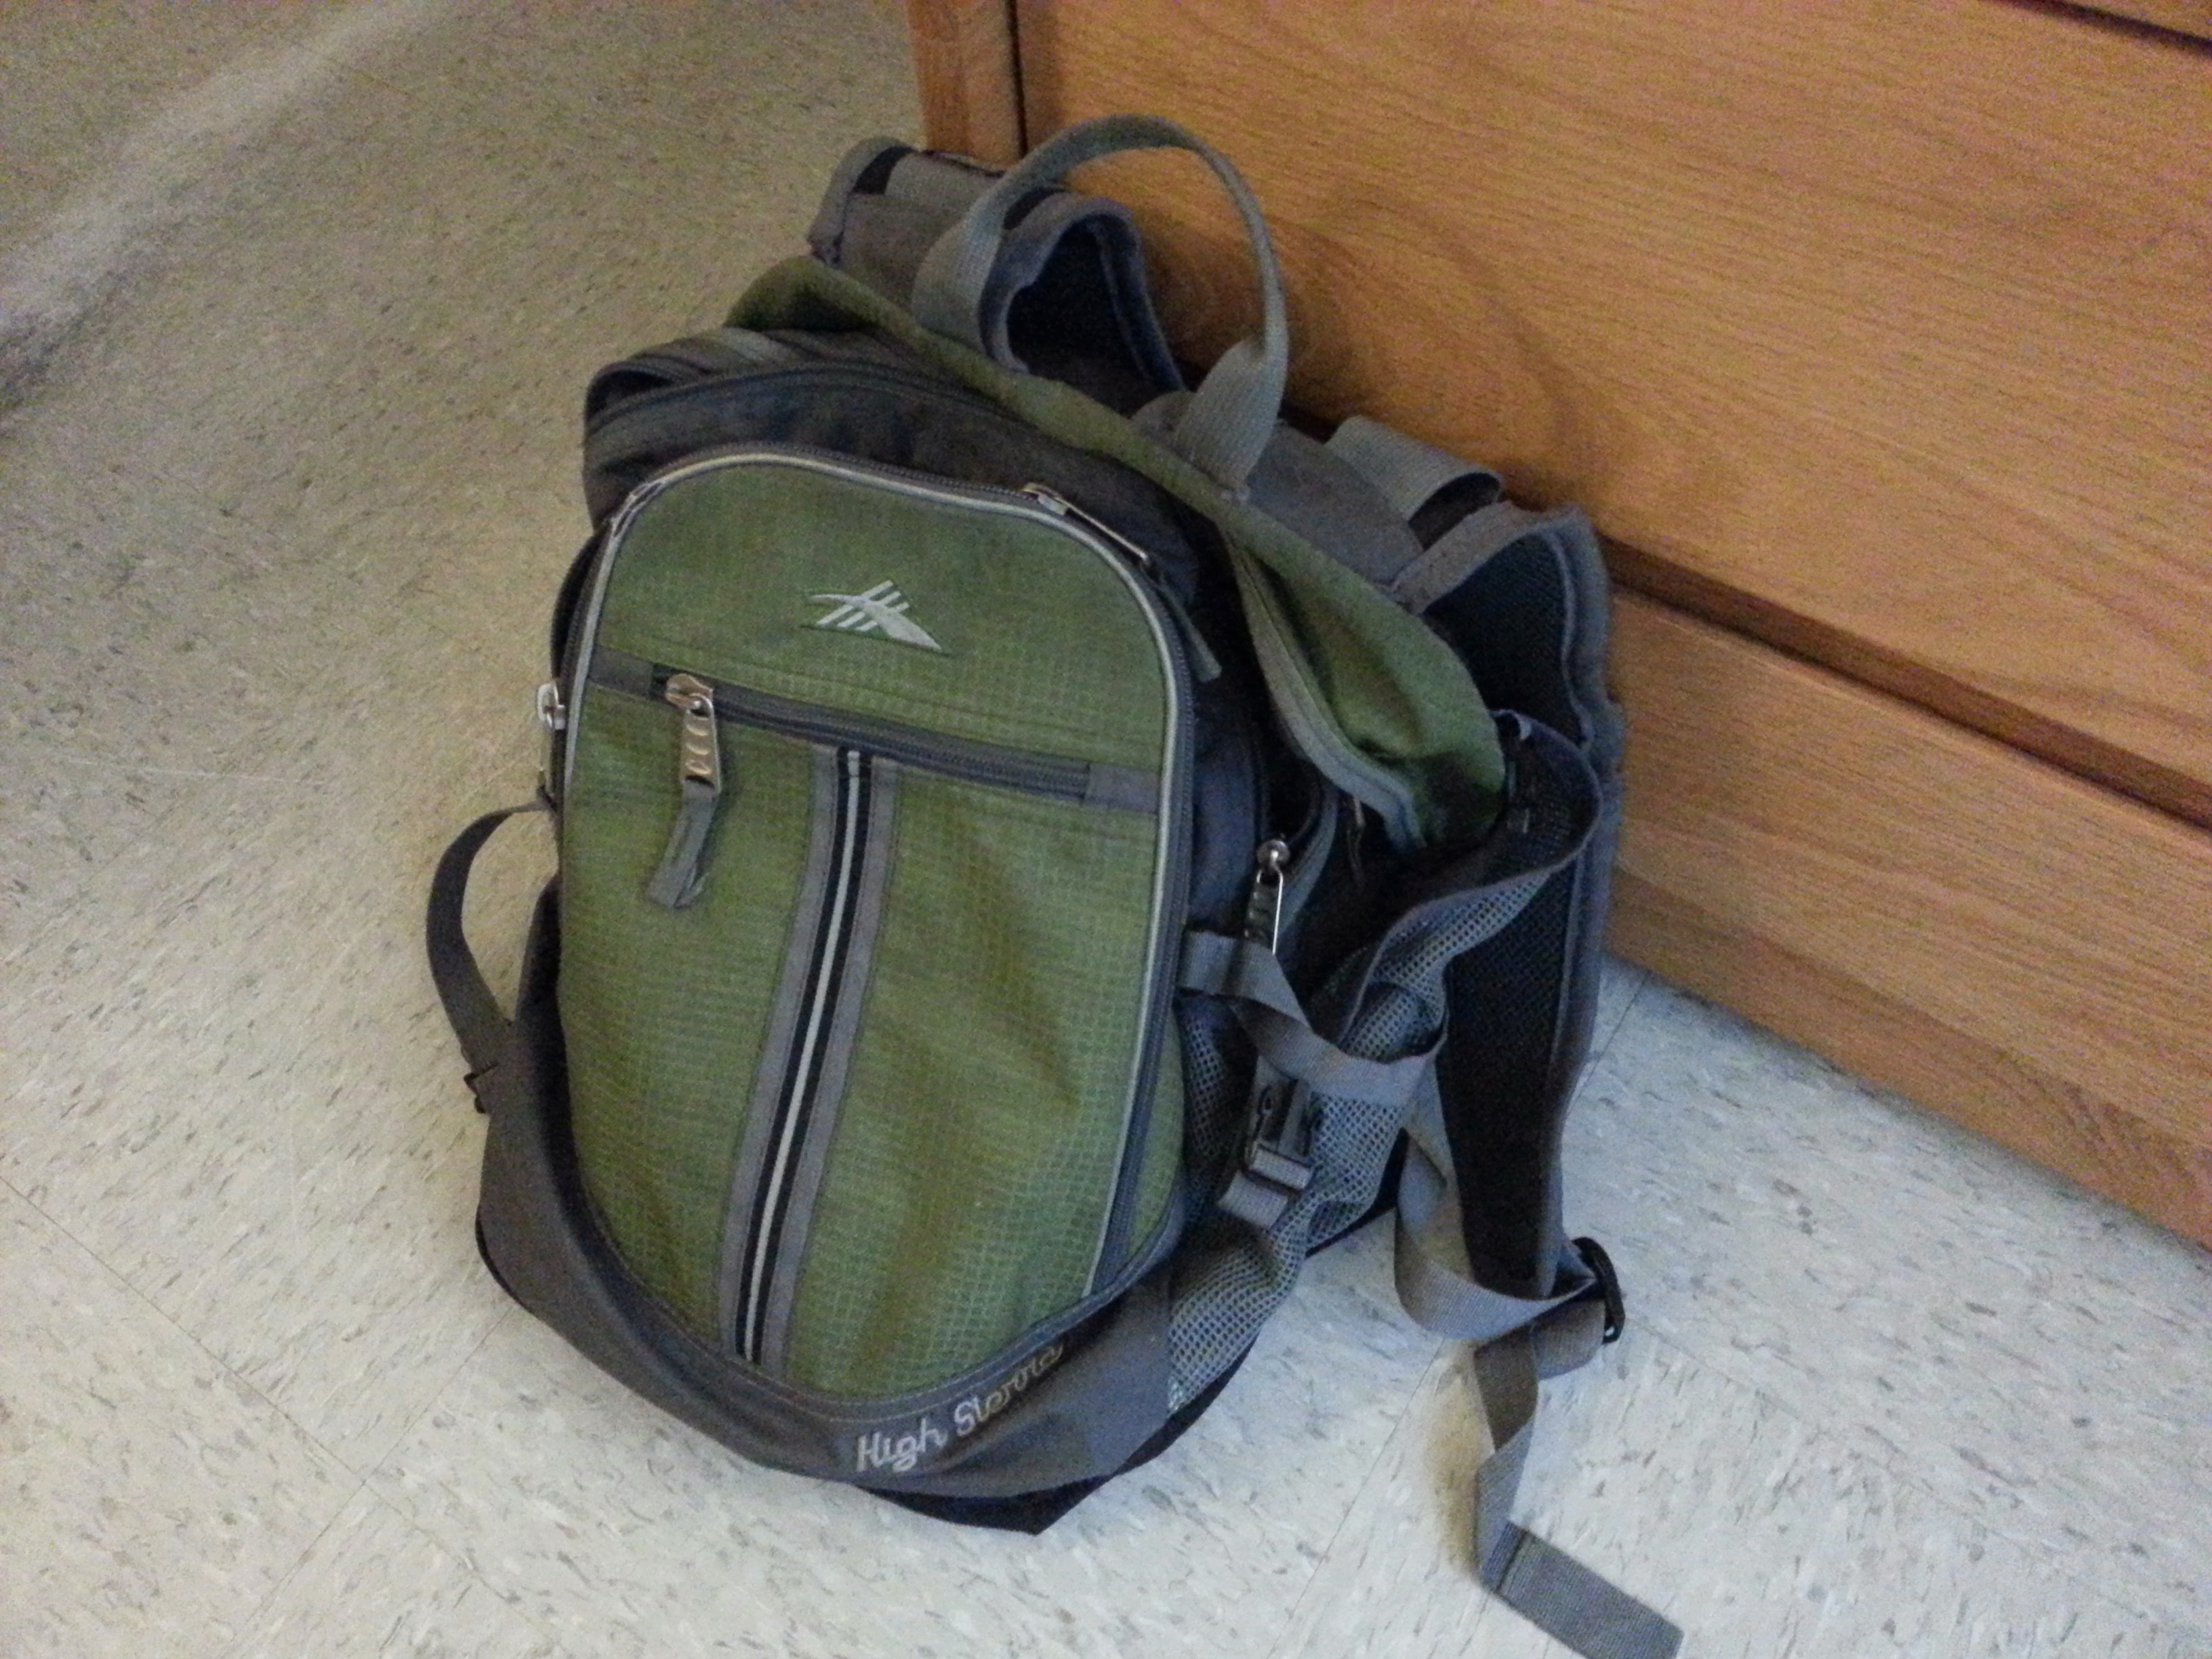
\includegraphics[width=3in]{images/backpack}
  % \caption{Sample illustration.}
% \end{figure}

\section{Planar depth reconstruction}

This is how planar depth reconstruction works!

\section{Results}

Talk about results.

Also talk about limitations.

\section{Conclusion}

In this paper, I have described the implementation of a system for
reconstruction of a planar representation of dense depth maps from multiple images
with an application to image-based rendering.

\bibliographystyle{acmsiggraph}
\bibliography{template}
\end{document}
